\documentclass[12pt, a4paper]{scrartcl}
\usepackage[utf8]{inputenc}
\usepackage{graphicx}
\usepackage{amsmath, amsthm, amssymb, textcomp}
\usepackage{setspace}
\usepackage{paralist}
\usepackage{graphicx}
\usepackage{caption}
\usepackage{epsdice}
\graphicspath{{WSK_im/}} %Graphic is in a folder named WSK_im in the currend directory
\usepackage{float}
\usepackage{authblk}
\renewcommand\Authfont{\fontsize{12}{14.4}\selectfont}
\title{Bayesian probability theory - Lesson 3:\\
Multivariate distributions - more Bayesics}

\author{Wolfgang von der Linden, Gerhard Dorn, Johanna Moser}
\date{Transcript}

\begin{document}
\setlength{\parindent}{0pt}
\maketitle
\onehalfspacing

Welcome to the third unit of the course Bayesian probability theory. 
My name is Wolfgang von der Linden and I will enable you to help 
Captain Bayes and her crew to investigate probabilistic problems involving more than one random variable. We will come to discuss \textbf{joint}, \textbf{conditional} and \textbf{marginal probabilities} and \textbf{in turn correlations}.
The aim of this unit is to discuss probabilistic problems from an enhanced perspective. 
We will learn how to include additional features into the description of an inference problem. 
That will allow us to update our state of knowledge based on additional information or experiments.
The introduction of several random variables will seamlessly lead to the second fundamental rule in probability theory: \textbf{the product rule}.
The question of Captain Bayes about the distribution of a sum of random variables will lead us to the \textbf{central limit theorem}.
Finally we will identify the rules of probability theory as the general calculus of propositions.\\


In the previous lesson we have discussed characteristics like mean and variance of probability distributions, that rely on one variable.
In this session we extend our language to problems where more than one random variable is concerned. We combine them into a \textbf{tuple} $P(X,Y)$  which often has the properties of a vector. Each of the components of the tuple or vector describes a different feature of the experiment or generally of the \textbf{inference problem}.
\section*{Joint probabilities}
\begin{figure}[H]
	\centering
	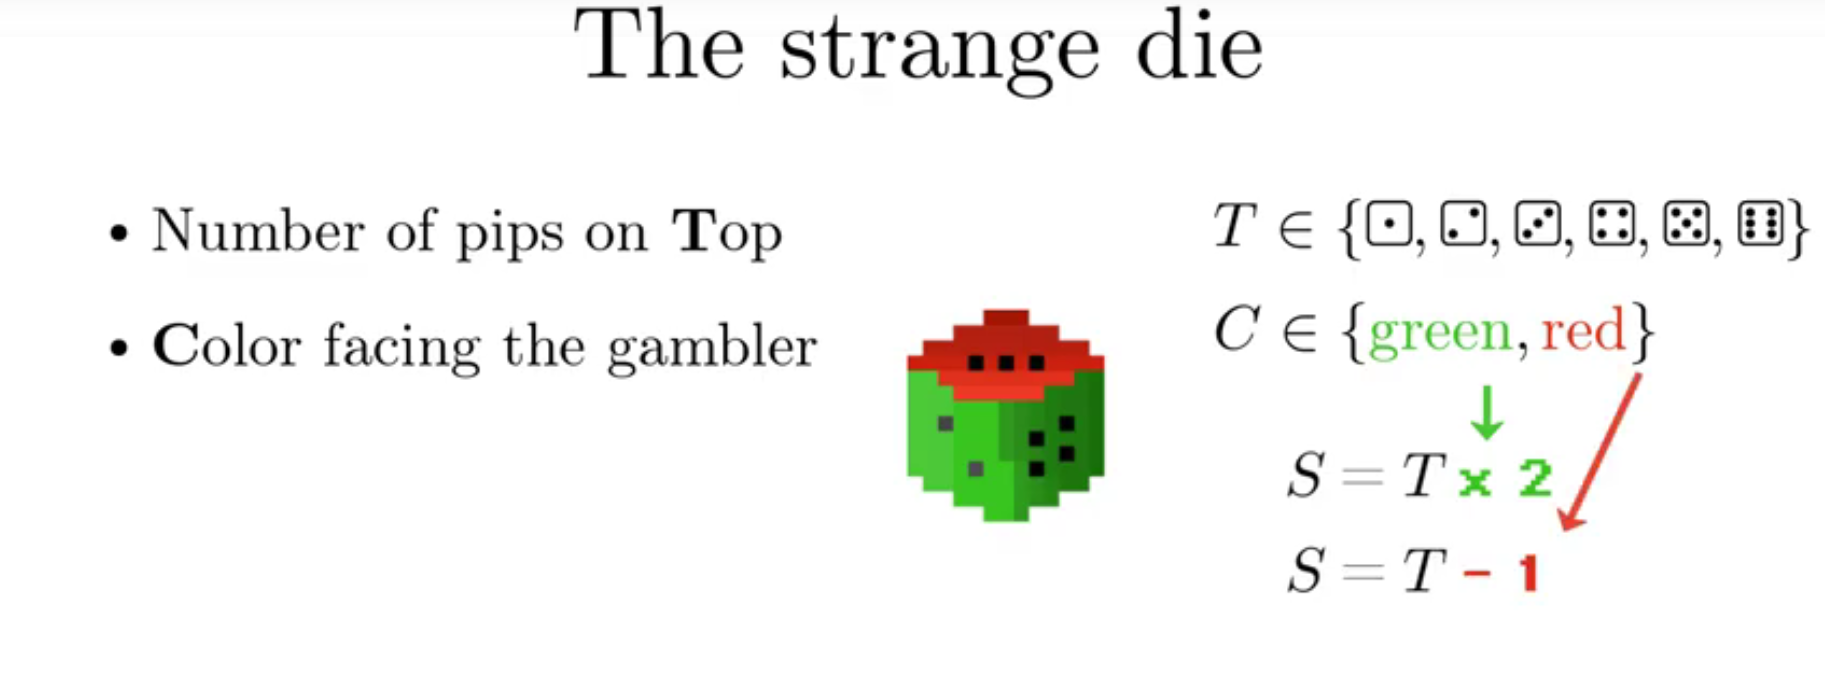
\includegraphics[width=0.75\textwidth]{3_1.png}
\end{figure}
For example, the strange die has two features that are important for the final score, namely the number of pips on top and the color of the front side, the one facing the gambler.
The front color is used as a modifier for the number of top pips, with green doubling the number and red reducing it by one.\\

\fbox{\parbox{\linewidth}{\textbf{Question 1.} What is the score $S$ of the feature pair (\epsdice{2}, green)?\\
a) 3 points\\
b) 5 points\\
c) 2 points\\
d) 1 point\\
e) 4 points
}}\\

Now we can describe the outcomes of the strange die by the tuple of these two features: top pips and front color. For instance \epsdice{5} and \textit{red}. In the latter case, the score is 4 points.
Note that the sample space consists of these feature pairs and they now \textit{form the elementary events}. It is a matter of perspective!
All in all there are 6 times 2, or 12 possible such feature pairs.
Note also that the score is a random variable that ranges from 0 to 12, but not all integers in this range are realized. 
Since a die has four side faces, you could also use more colors and different rules to invent your own strange die game.\\
\begin{figure}[H]
	\centering
	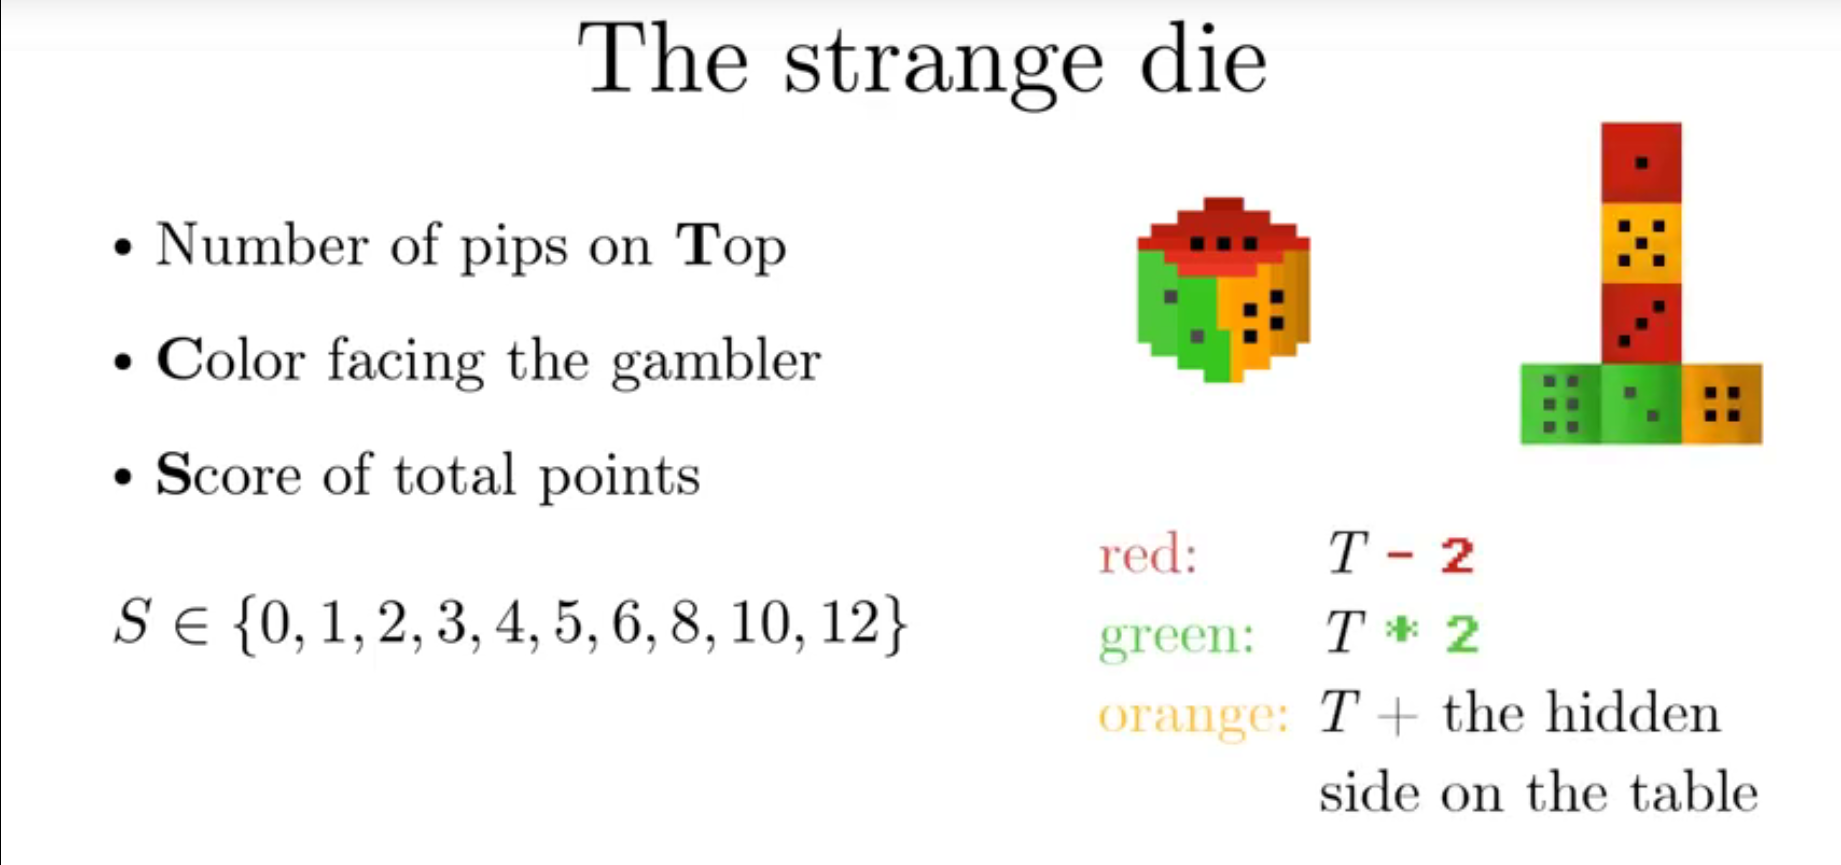
\includegraphics[width=0.75\textwidth]{3_2.png}
\end{figure}
\fbox{\parbox{\linewidth}{\textbf{Question 2.} Look at the cube net of the three colored strange die. Which of the following statements are true?\\
a) When having four pips on tom ($T=$ \epsdice{4}), I get the highest score $S$ when an orange face is pointing at me (i.e. the gambler).\\
b) The combination (\epsdice{1}, red) is not possible.\\
c) It is more likely to have a green or orange side facing the gambler than having a red one.\\
d) The lowest possible score is $S=-1$.
}}\\

Next we want to assign probabilities to the scores:
Laplace colored the faces of the die \textit{green for an even} and \textit{red for an odd number of pips}. 
The die Bernoulli and Laplace are using for the trinautic tournament is strange because the pips are arranged in an unusual way. We illustrate this by a net of the cube. 
\begin{figure}[H]
	\centering
	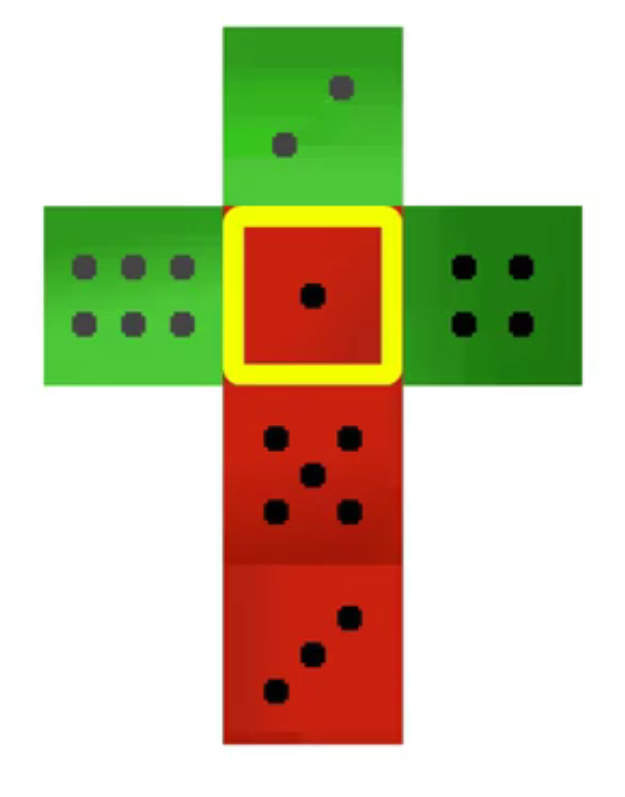
\includegraphics[width=0.35\textwidth]{3_3.png}
\end{figure}
The yellow framed face represents the top of the die, showing the number \epsdice{1} in this example.
The four faces surrounding it are the possible candidates for the sides pointing towards the gambler. Note that there are in total 6 times 4, or 24 possible geometric realizations of the die experiment if you take the side face orientation also into account.
In order to assign probabilities we count the geometric realizations that lead to a defined feature pair of top pips and front color.
In this example with one pip (\epsdice{1}) on top we count 3 realizations for the green and 1 realization for the red modifier.
Similarly we proceed with the other values for the top pips: \epsdice{2}, \epsdice{3}, \epsdice{4}, \epsdice{5} and \epsdice{6} and obtain the following table. %3_4
\begin{figure}[H]
	\centering
	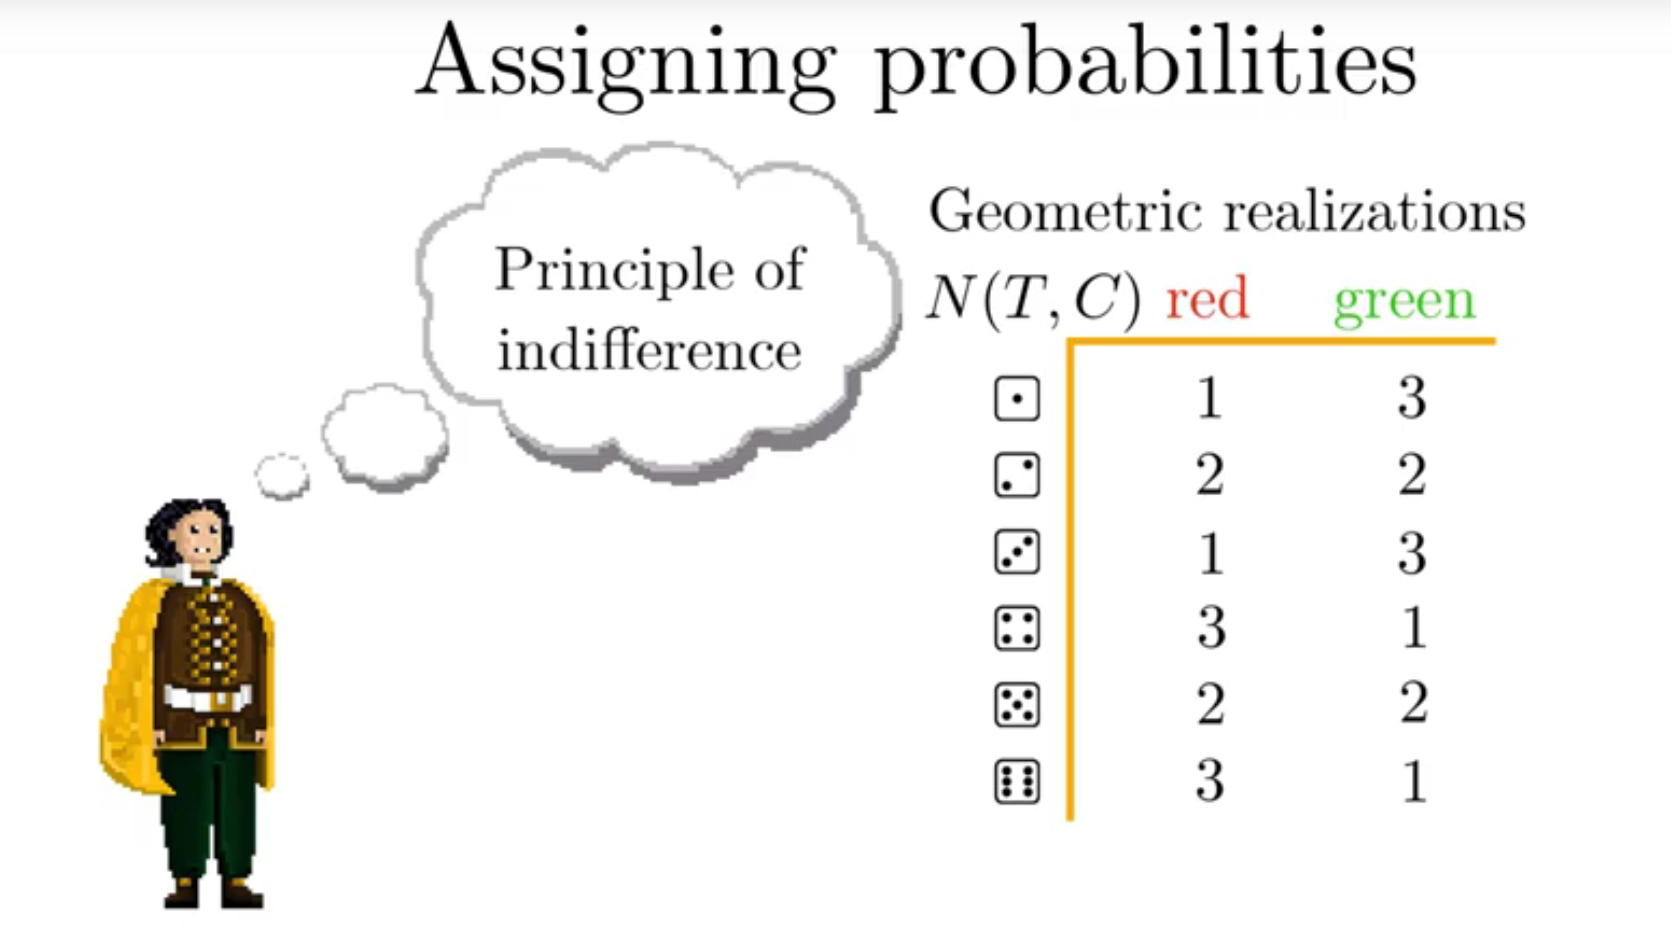
\includegraphics[width=0.75\textwidth]{3_4.png}
\end{figure}
According to the \textbf{principle of indifference} all geometric realizations are equally probable and therefore the classical assignment of probability for a pair (top pips, front color) is given by the \textit{number of favorable geometric realizations} - which are the numbers in the table - \textit{divided by total number of geometric realizations}, which is 24. 
The probability for the pair \epsdice{6} and red is therefore 3 divided by 24 resulting in 12.5 \%.  \\

\fbox{\parbox{\linewidth}{\textbf{Question 3.} What is the probability of the feature pair (\epsdice{2}, green)?\\
a) 25\%\\
b) 1/24\\
c) 8.3\%\\
d) 12.5\%
}}\\

That leads to the following table of \textbf{joint probabilities}. %3_5
\begin{figure}[H]
	\centering
	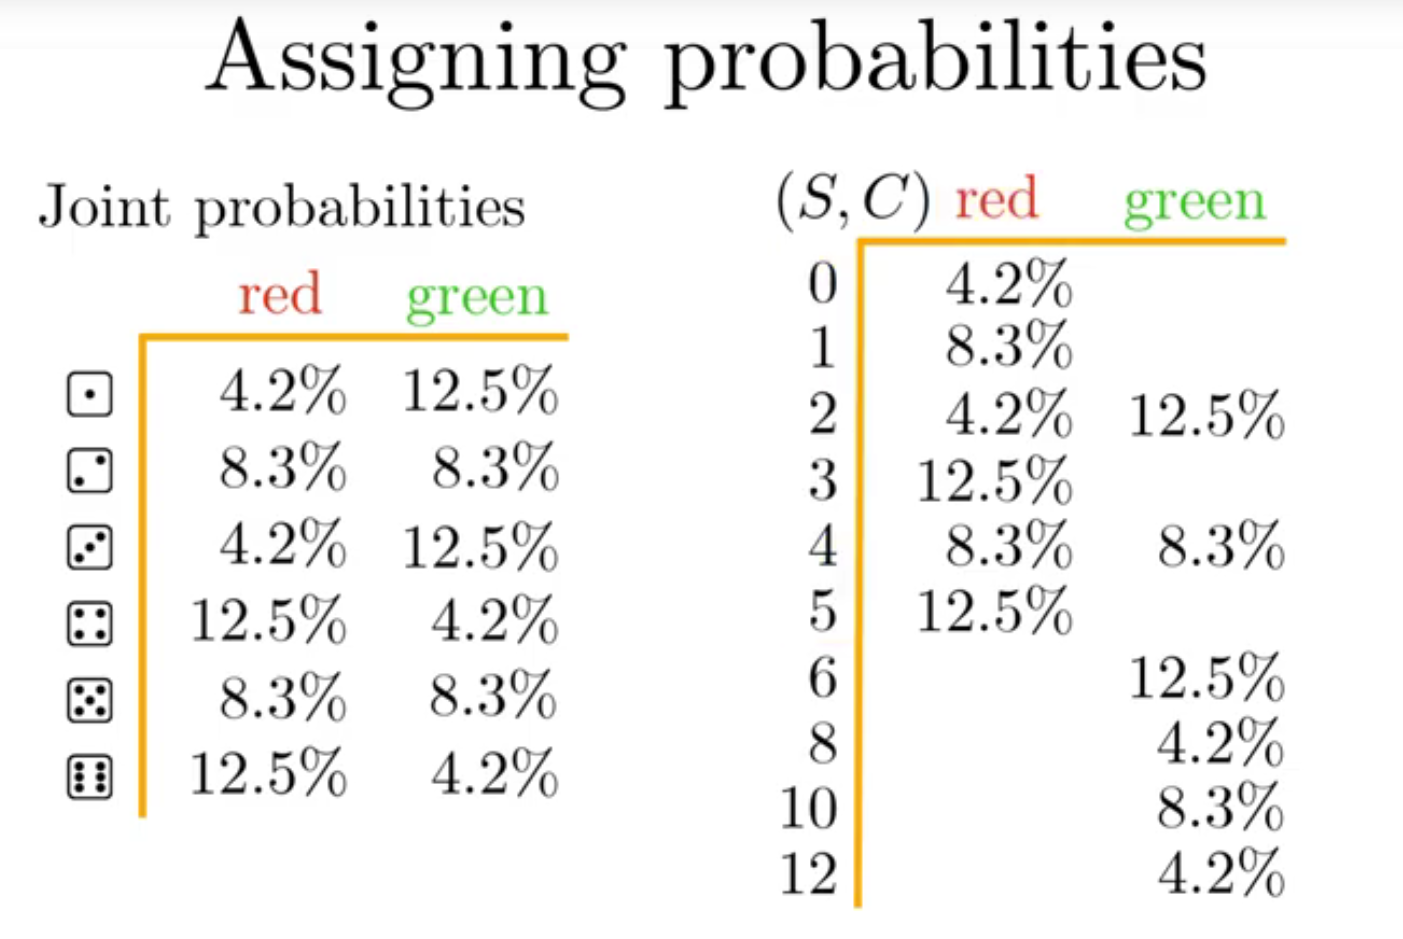
\includegraphics[width=0.75\textwidth]{3_5.png}
\end{figure}
From the table of joint probabilities for the feature pairs we can easily construct another representation, namely the pair ``score and front color''.
If the font color is green, the score is obtained by multiplying the top pips by 2.
Likewise, if the front color is red, the score is obtained by reducing the top pips by one.
These tables represent different joint probabilities. 
Needless to say that joint probabilities can also be defined for more than two propositions or variables $P(A,B,C,\ldots)$.\\

\section*{Conditional probabilities}
Now that we know the joint probabilities, there are different aspects of the inference problem that we can be address.
In case of the strange die, we could ask the question:  
``\textit{What is the probability for a particular score, for example 6 points, given the front side is green?}''.
Such an object is called \textbf{conditional probability}, since one feature - here the color - is \textit{fixed}. 
We use a vertical line to separate the random variables or events of interest from the fixed conditions. In terms of propositions the notation is shorter, $P(A|B)$ describes the probability for $A$ given $B$ is true for sure.
When we examine the probabilities for all values of the random variable score, given that the color is green, we obtain the \textbf{conditional probability distribution}.\\

\fbox{\parbox{\linewidth}{\textbf{Question 4.} Fill in the gaps correctly (``a variable", ``the conditional bar", ``a conditional probability", ``a conditional probability distribution", ``an outcome")\\
The term $P(X_i|\text{red})$ is a .......... whereas $P(X|\text{red})$ is .......... since the first argument is .......... in the first place and .......... in the second.\\
Note that you always find an event, a proposition, or an outcome behind ............ .
}}\\

We want to illustrate this concept on the strange die and compute the conditional probability $P(S|\text{green})$.
Note that the sample space has shrunk as only the elements with green front face are considered.
The elements that we consider are the same as those in the joint probability. Therefore the probability ratios between them have to be the same.
Consequently, the \textit{conditional probability is proportional to the joint one} in other words, only the \textbf{normalization} $Z$ has changed which is now given by \textit{summing the joint probability} of the score values resulting in the depicted table.\\

\fbox{\parbox{\linewidth}{\textbf{Question 5.} What is the value of the normalization $Z$ in this case: $$Z=\sum_iP(S_i|C=g)$$\\[-1cm]
a) 0.5\\
b) 1/24\\
c) 25\%\\
d) 12.5\%
}}\\[0.2cm]
Similarly, we obtain the conditional probabilities for the score given the front color is red.\\ %3_6
\begin{figure}[H]
	\centering
	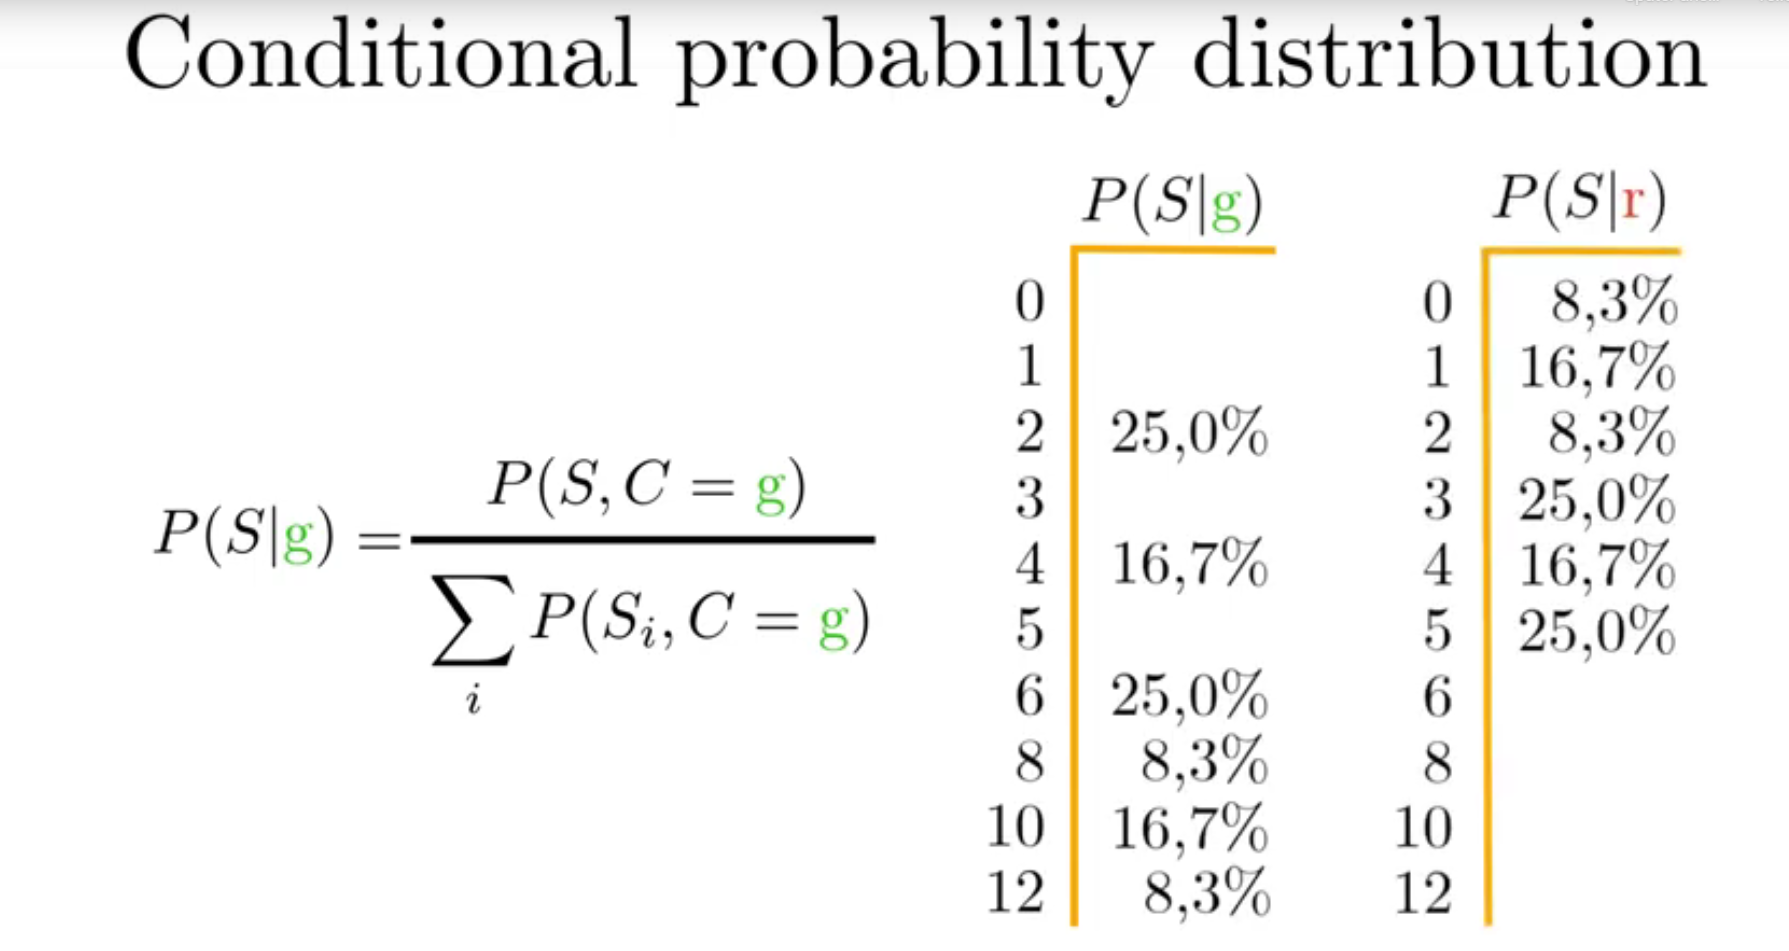
\includegraphics[width=0.75\textwidth]{3_6.png}
\end{figure}

Now we change the perspective into the opposite. Instead of fixing a feature we simply don’t care about it.
For example we might want to know the probability for the score being 4, say, irrespective of the front color or we are interested in the probability that the front color is green, irrespective of the number of scores.
We use again the table of joint probabilities and consider the joint feature pair (score and color) as elementary event. 
For \textit{fixed score S}, the events with the same score but different colors are exclusive and therefore the \textbf{simplified sum rule} $P(S_1 \text{ or } S_2)=P(S_1)+P(S_2)$ applies. %sum rule
On the other hand, from \textbf{boolean algebra} we know that the argument of the left hand side turns out to be the score. 
In our example, we obtain the probability of a certain score just by \textit{summing the rows} and noting the resulting probability on the right margin.
Similarly, we obtain the marginal probabilities for the colors by \textit{summing the columns} of the table.
Thereby, we find  $P$(red) is equal to $P$(green) is equal to $0.5$. %3_7
\begin{figure}[H]
	\centering
	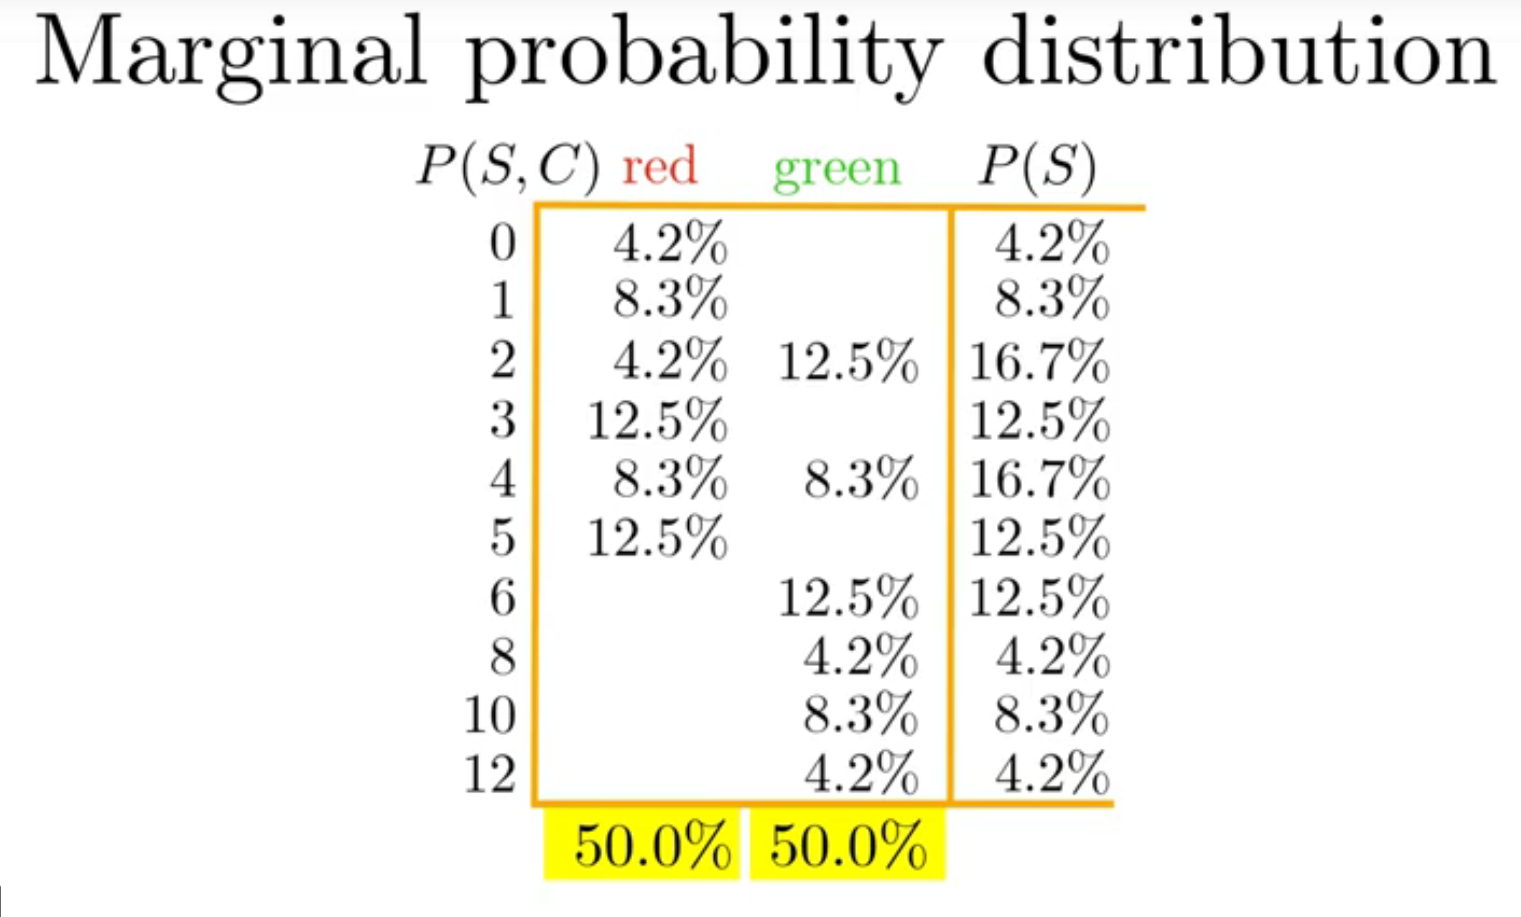
\includegraphics[width=0.75\textwidth]{3_7.png}
\end{figure}

\fbox{\parbox{\linewidth}{\textbf{Question 6.} Do you see an easy explanation for this result?\\
a) The dice has 3 green and 3 red faces so the probability for green, as well as the probability for red, is 0.5.\\
b) The cube net of the problem was chosen in such a way that the probability for green adds up to 50\%. The probability for red follows from the sum rule.\\
c) The four side faces can have two different colors. In total, we find green faces and two red ones on average.
}}\\
\section*{Marginal probability}
This brings us to the \textbf{marginalization rule} in its most general form: 
We consider any set of  \textbf{complete} and  \textbf{exclusive} propositions $B_i$, which means they form a \textit{non-overlapping partition of the sample space}.
Then we obtain the generalized marginalization rule.
\begin{equation*}\boxed{P(A)=\sum_iP(A,B_i)}\end{equation*}
The importance of this rule cannot be overestimated.
Again, a generalization to more than two variables is given by multiple sums.\\
\fbox{\parbox{\linewidth}{\textbf{Question 7.} Let's try to apply the marginalization rule. Which example applies it correctly?\\
a) $P$(g)=$P$(g, even number of pips) + $P$(g, uneven number of pips)\\
b) $P$(\epsdice{3}) = $P$(\epsdice{3}, g) + $P$(\epsdice{3}, r)\\
c) $P$(g) = $P$(g, $>$ \epsdice{3}) + $P$(g, $\leq $ \epsdice{2})\\
d) $P$(\epsdice{5}) = $P$(\epsdice{5} $|$ g) + $P$(\epsdice{5} $|$ r)\\
e) $P$(g) = $P$(g, odd number of pips) + $P$(g, $\geq$ \epsdice{2})\\
f) $P$(g) = $P$(g, \epsdice{3}) + $P$(g, $\lnot$ \epsdice{3})
}}\\

\section*{The product rule}
Now we come to the second fundamental rule of probability theory, the  \textbf{product rule}.
We combine the formula we obtained for the conditional probability and the formula for the marginal probability and obtain $P(S_j|g) = \frac{P(S_j, g)}{P(g)}$ 
Written differently, we obtain the famous product rule, which has the general form. 
\begin{equation*}\boxed{P(A,B)=P(A|B)P(B) = P(B|A)P(A)}\end{equation*}
Note that $A$ and $B$ do not have to be elementary events or be assigned to random variables but can be \textit{arbitrary propositions}.
The product rule enables us to change the perspective of an inference problem, since it is the formula that links  \textbf{assumptions} - propositions behind the conditional bar - with  \textbf{open questions} - propositions before the conditional bar. We will see in unit 6 how this product rule enables us to swap assumption and open question to tackle inverse problems.
Note, that for \textit{uncorrelated} propositions $A$ and $B$ the product rule simplifies to $P(A,B)=P(A)P(B)$, like the probability for rain and rolling six pips on a die is equal to the product of the two probabilities.\\

\fbox{\parbox{\linewidth}{\textbf{Question 8.} Let's apply the product rule! Which of the following equations describe the application of the product rule?\\
a) $P(\epsdice{6},\,$g) = $P$(\epsdice{6}$\,|\,$g)$\, \cdot\, P$(\epsdice{6})\\
b) $P$(\epsdice{4}) = $P$(\epsdice{4}$\,|\,>$ \epsdice{3})$\, \cdot\, P$($>$ \epsdice{3})\\
c) $P(\text{r},\,$\epsdice{4}) = $\frac{P(r,\, \epsdice{4})}{P(\epsdice{4})}$\\
d) $P$(\epsdice{3}$\,|\,$r)$\, \cdot\, P$(r) = $P$(r$\,|\,$\epsdice{3})$\, \cdot\, P$(\epsdice{3})\\
e) $P(\epsdice{2},\,$g) = $P$(g$\,|\,$\epsdice{2})$\, \cdot\, P$(g)
}}\\

It was a long and winding road in the history of science until this general form could be proven rigorously.
It is applicable to the most general definition of probability as a \textit{measure for the truth of a proposition}.
Then probability theory can be considered as calculus of propositions and is a seamless generalization of Boolean algebra to partial truth.
The only axioms this calculus is based on are  \textbf{consistency}, which means, one gets the same result no matter along which path a calculation is performed, and  \textbf{continuity} with respect to small changes of parameters.
If there are more than two propositions, there are several choices of propositions for which we can compute the probabilities conditional on the others - corresponding to different perspectives of the problem.\\

\section*{The conditional complex}
Note: \textit{There is no such thing as an unconditional probability, it always relies on assumptions}.
Like the die is perfectly symmetric, the throw guarantees a chaotic trajectory, the players are not cheating, the die has six faces. It will never land on an edge or corner and so on.
We combine all these assumptions in the so called  \textbf{background information}.
We do not always write the background information explicitly, but keep in mind that it \textit{has to be fixed} and \textit{cannot be changed} during the calculations to remain consistent since you cannot expect the same outcome of an experiment when you alter its setup.
If some assumptions may be altered (new information, looking at different aspects) then we will write them explicitly behind the conditional bar. 
As a matter of fact, the background information is nothing but a proposition, and one is immediately prompted to move it in front of the conditional bar. 
That allows to check our assumptions, like what is the probability that a coin is fair, if it lands heads up ten times in a row. $P$(10 heads in a row $|$ coin is  fair)$ \Rightarrow$ $P$(coin is fair $|$ 10 heads in a row row)= ?
But you'll have to be patient - we will cover this topic only in a later unit.\\


So far, we have discussed three different aspects of probability distributions, joint, marginal and the conditional probability.
Now we want to turn to the computation of  \textbf{mean values} for these cases. In the adventure of Captain Bayes the question was raised about the average score obtained in the strange die game. One way to compute it, is to define the function $S(T,C)$ that evaluates the score from the number of top pips and the front color. Then the average score is given by the \textit{sum of this function times the joint probability}.\\
\begin{equation*}\boxed{\langle S(T,C)\rangle= \sum_{ij}S(T_i,C_j)P(T_i,C_j)}\end{equation*}\\
%3_8
\begin{figure}[H]
	\centering
	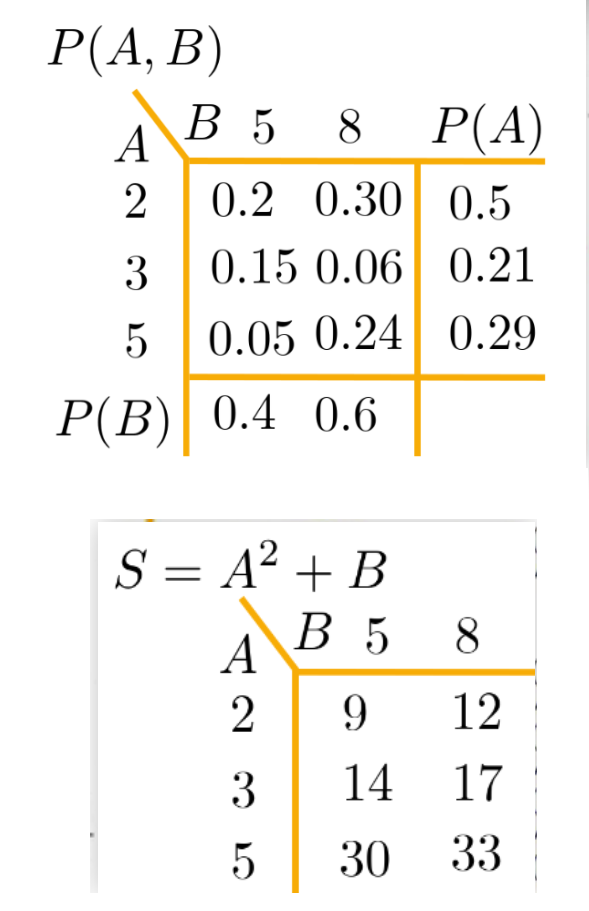
\includegraphics[width=0.35\textwidth]{3_8.png}
\end{figure}
\fbox{\parbox{\linewidth}{\textbf{Question 9.} Calculate the mean value of the score.\\
The mean value of the score $S=A^2+B)$ given by the probability distribution $P(A,B)$ in the two tables above is $\langle S\rangle =$........
}}\\

Alternatively, we could use the marginal probability mass function for the score $\sum_iS_iP(S_i)$, which we computed already, resulting in $4.5$.
Finally, we can address Laplace’s question concerning the average score he gets, assuming he always sees the green front face. In this case the answer is given by the mean value of the conditional probability distribution $\langle S \rangle _{|\text{g}} = \sum_iS_iP(S_i|\text{g})$ resulting in six points on average.
Quite similarly we obtain the averaged conditional on red to be three.\\
%3_9
\begin{figure}[H]
	\centering
	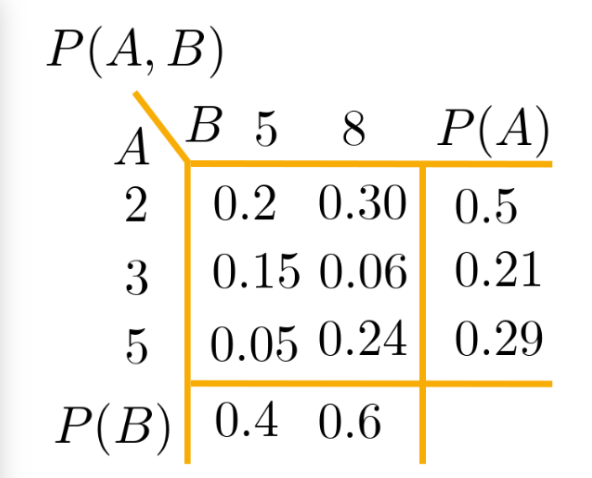
\includegraphics[width=0.35\textwidth]{3_9.png}
\end{figure}
\fbox{\parbox{\linewidth}{\textbf{Question 10.} Calculate the requested values using the table above.\\
The normalization needed to get the conditional probability distribution $P(A|B=5)$ is $Z_{B=5}=$........\\
The conditional mean value $\langle A \rangle_{B=5} =$.......\\
The conditional mean value $\langle B \rangle_{A=2} =$.......
}}\\
Often times, the conditional probabilities and their means are more easily accessible than the joint probabilities, in which case we can employ a useful expression for the total mean.
\begin{equation*}\boxed{\langle S\rangle= \sum_{i}\langle S\rangle_{C_i}P(C_i)}\end{equation*}\\
Applied to the strange die, we then find the result in agreement with the previous result.
All of the above considerations can readily be generalized to other problems with two random variables.\\%3_10
\begin{figure}[H]
	\centering
	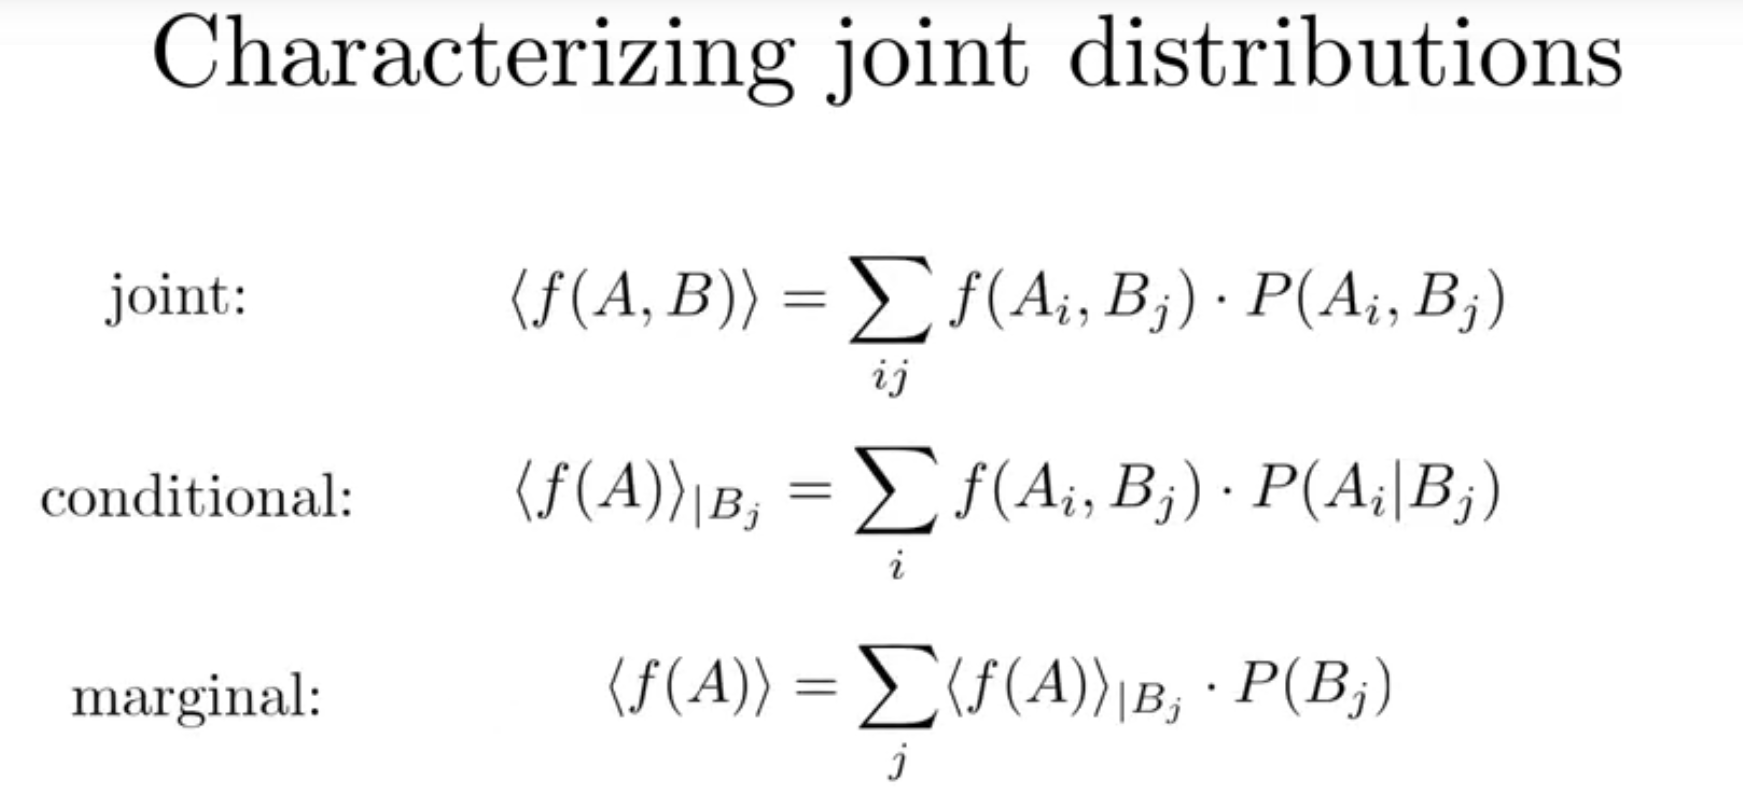
\includegraphics[width=0.75\textwidth]{3_10.png}
\end{figure}

The  \textbf{variance} is in principle just a special case of the previous discussion. But due to its importance we will give the result explicitly. We compute it for the score of the strange die for which we need $\langle S^2\rangle - \langle S\rangle ^2=8.9$.\\ 

\section*{Covariance}
Another important object in the analysis of random variables or generally in inference problems is the  \textbf{covariance} which allows to identify correlations between different features $A$ and $B$. 
%3_11
\begin{figure}[H]
	\centering
	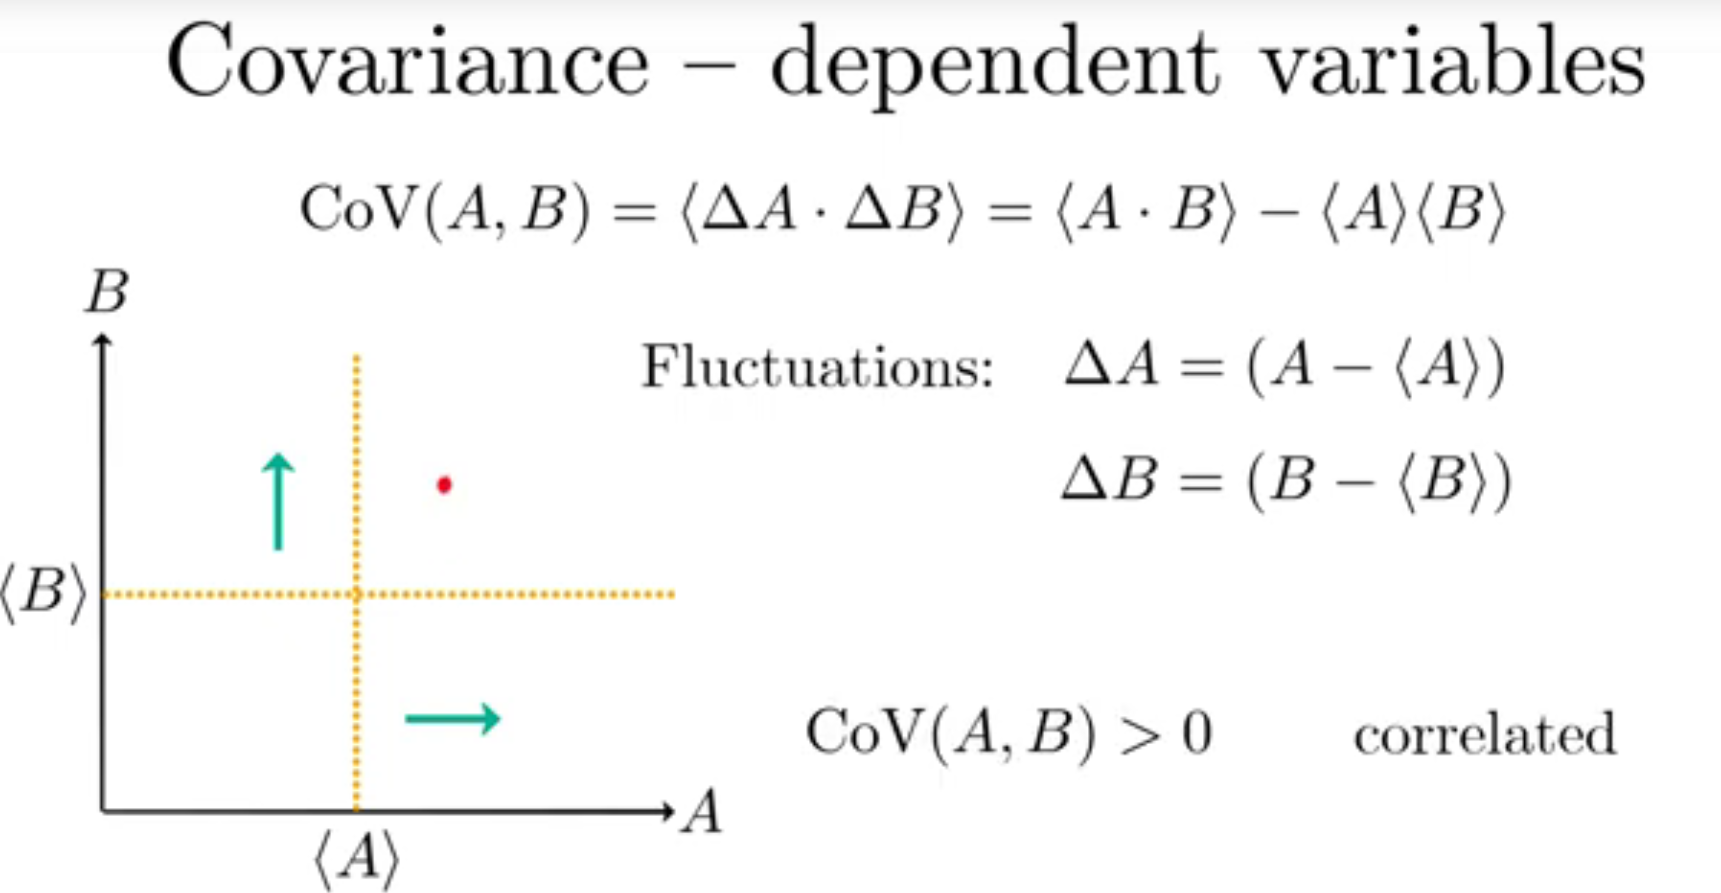
\includegraphics[width=0.75\textwidth]{3_11.png}
\end{figure}
It shows whether on average an \textit{increase of A (above its mean) is associated with an increase of B (above its mean) or whether it is associated with a decrease of B (below its mean)}. 
For example, we could test whether, in a population, a person's weight is correlated or anti-correlated with his or her height.
If \textit{fluctuations of one feature are independent of fluctuations of the other feature} then the covariance is  \textbf{zero}. 
That implies according to its definition that the \textit{mean of a product is the product of the means} and, therefore, the joint probability factorizes into the product of the marginal probabilities.
\begin{equation*}\boxed{\text{CoV}(A,B)=0 \Rightarrow \langle AB\rangle = \langle A\rangle\langle B\rangle \\
\Rightarrow P(A,B) = P(A)P(B)}\end{equation*}\\
Now we can apply the covariance to examine Pascal's notes on the sailing deviations. Since we have measured data, we can estimate the joint probabilities by the relative frequencies. As discussed along with the sample variance we have to correct for a bias due the use of the sample mean value.%3_12
\begin{figure}[H]
	\centering
	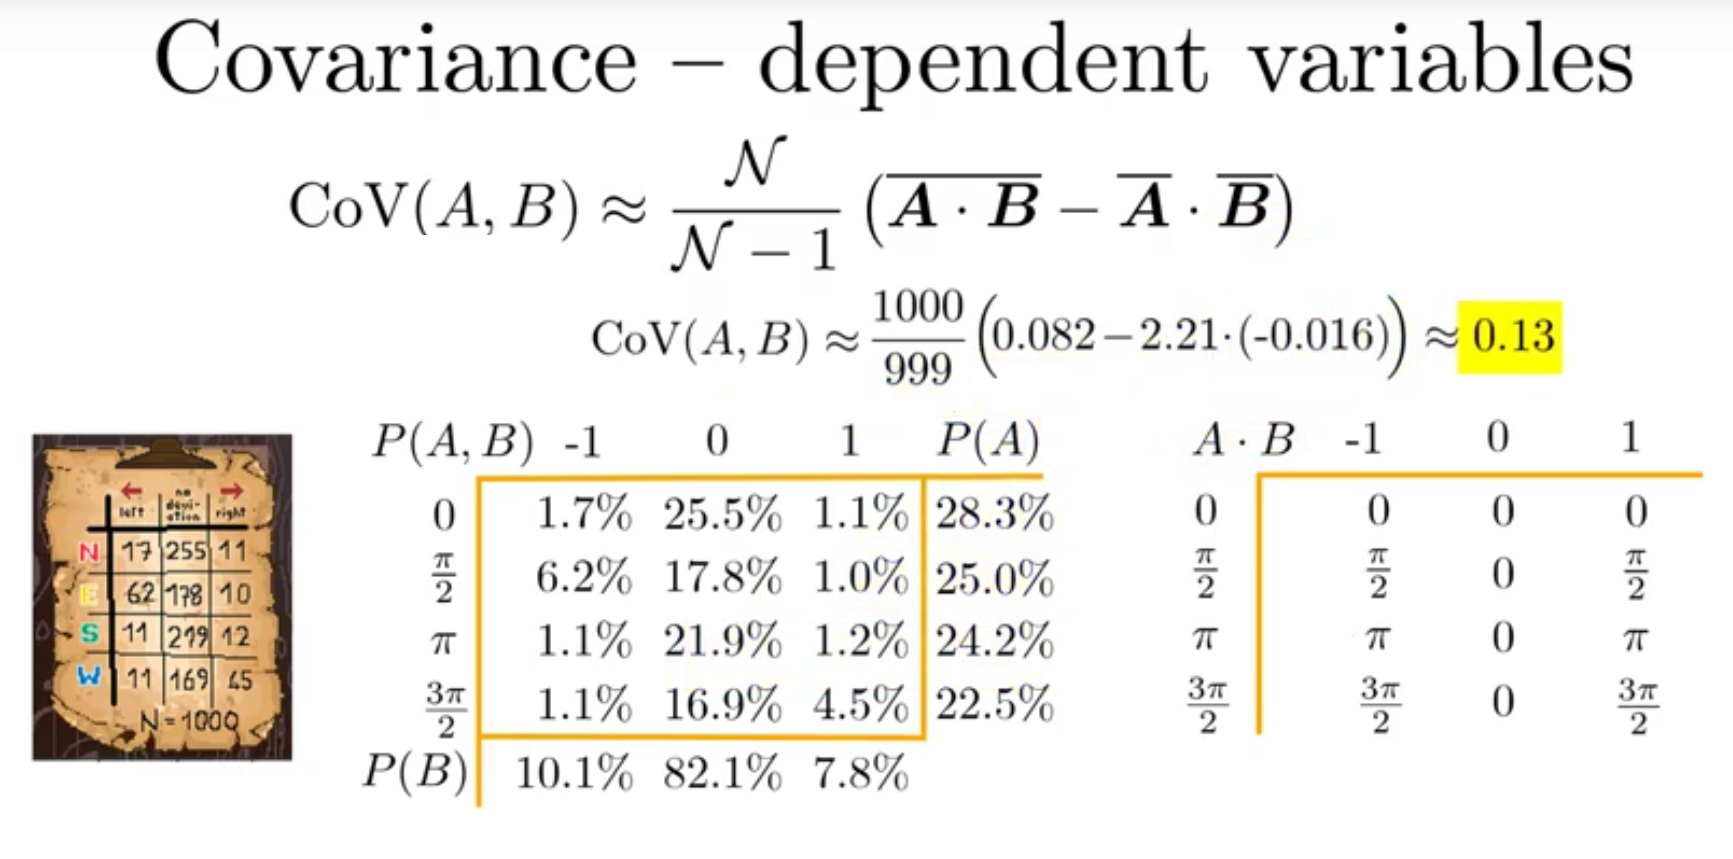
\includegraphics[width=0.75\textwidth]{3_12.png}
\end{figure}
The covariance of the sailing direction and the sailing deviation  of Pascal’s notes is $0.13,$ indicating a correlation between sailing direction and deviation, which can be considered as a hint for the presence of an ocean drift.
All what we have discussed so far can readily be generalized to more than 2 features, variables or rather propositions.\\%%

\section*{The central limit theorem}
In the adventure Bayes was wondering how the sum of the strange-die-scores of her crew might be distributed. This brings us to the  \textbf{central limit theorem (CLT)}. 
The scores of the crew-members are actually random variables.
Let’s be flexible as to the size of the crew and just denote it by N.
The individual random variables have special properties: 
They are  \textbf{Independently and Identically Distributed} which is abbreviated by ``i.i.d.".
What does that mean?\\
\textbf{Identical} means that \textit{all random variables have the same probability mass function}, characterized by its mean and variance.
 \textbf{Independent} means uncorrelated and implies that the \textit{covariance between different variables is zero}. 
Now we turn to the averaged total score, as that is what we are really interested in.
We call it  \textbf{arithmetic mean}, although the objects are random variables.
\begin{equation*}\boxed{T = \frac 1N \sum_iS^{(i)}
}\end{equation*}\\
It should be obvious that $T$ is also a random variable. 
For the mean of $T$ we obtain from the previous slide and the linearity property that it is identical to the mean of the distribution of the individual terms.
\begin{equation*}\boxed{\langle S^{(i)} \rangle = \mu \Rightarrow \langle T\rangle = \mu
}\end{equation*}\\
The variance of $T$ is given by variance of the distribution of the individual terms divided by $N$.
\begin{equation*}\boxed{\text{Var}(T)=\frac{\sigma^2}{N}
}\end{equation*}\\
Even more thrilling is what Captain Bayes wanted to know, namely the detailed form of the distribution of $T$. The central limit theorem states that the probability distribution of $T$, being the mean of $N$ Independently and Identically Distributed random variables approaches the  \textbf{Gaussian distribution} for $N$ going to infinity with mean and variance given before.
\begin{equation*}\boxed{\lim_{N\rightarrow \infty} T \approx \mathcal{N}\left(\mu, \frac{\sigma}{\sqrt{N}}\right)}\end{equation*}\\
So the distribution of $T$ universally approaches a distribution called  \textbf{"Gaussian"} irrespective of the shape of the probability mass function of the individual terms.\\
What is a Gaussian?
The Gaussian distribution is one of the most important and ubiquitous distributions in probability theory. It is given by the following formula and parameterized by mean and variance.
\begin{equation*}\boxed{
\mathcal{N}(X|\mu, \frac{\sigma}{\sqrt{N}})=\frac{1}{\sqrt{2\pi \sigma ^2}}\exp\left(-\frac{(X-\mu)^2}{2\sigma^2}\right)
}\end{equation*}\\
It has the shape of a bell and is thus often called  \textbf{bell curve} or  \textbf{Normal distribution}.
The limit $N$ going to infinity itself is actually not very relevant for most real world applications, but already for moderately large $N$ ($N\geq 30$) the distribution is confusingly similar to a Gaussian. 
So Captain Bayes will find that the distribution of the averaged score of her crew in the strange die game will look like a Gaussian.


This concludes the third unit. Investigate the sums of random variables and the central limit theorem using the interactive simulations,  feel free to ask questions in the forum and feel encouraged to test your knowledge in the quiz!



\vspace{2cm}
\begin{minipage}[t]{1\textwidth}
	\raggedleft
	\centering
	
\includegraphics[width = 0.20\textwidth]{CC-BY_icon}
	\vspace{0.2cm}
	
	\centering
	{\large ITPCP, TU Graz} \\
	https://creativecommons.org/licenses/by/4.0/legalcode
\end{minipage}


\end{document}